\chapter{Organisation du projet}

\section{Organisation du travail}
% auteur : Adrien
% relu par : Fabien, Florian, Clément, Thin

Nous avons rapidement opté pour une méthodologie SCRUM, alternant régulièrement réunions, phases d'analyse et phases de développement, avec une version à rendre à chaque réunion.

\subsection{Réunions de travail}

Des réunions de travail regroupant les membres du groupe ainsi que notre encadrant Jacques Ferber se sont tenues régulièrement au LIRMM.
 et ont vu se dérouler de nombreuses présentations d'outils et de propositions de directions à prendre.
Durant la phase de développement ces réunions ont été espacées de façon bimensuelle, afin de laisser le temps au groupe de réaliser une nouvelle version, et avaient pour but principal de définir l'avancement du projet et quelle direction il devait prendre aussi bien à court terme qu'à long terme.

D'autres réunions plus informelles se sont déroulées entre tout ou partie des membres du groupe en de divers lieux comme la Faculté Des Sciences ou le LIRMM, chacune répondant à un besoin spécifique.

\subsection{Répartition des tâches}

À la fin de chaque réunion, les membres choisissaient les tâches dont ils souhaitaient s'acquitter, ou prenaient les tâches restantes ainsi le travail était réparti et tous les membres du projet avaient des objectifs à réaliser pour la réunion suivante.

\subsection{Planification du développement}
% auteur : Fabien
% relu par : Florian, Clément, Thin

Le développement a été réalisé intelligemment, en effet, la méthode agile (fortement réputée dans le monde de l'entreprise) semblait être la plus propice pour la réalisation de ce projet. C'est pourquoi nous l'avons utilisée.
Ainsi, environ toutes les deux semaines (après un certain nombre de changements majeurs) une nouvelle version opérationnelle naissait. 
Le site est désormais hébergé, il est donc accessible en ligne (voir \cite{poavre}).

\subsection{Élection d’un chef de projet}
% auteur : Fabien
% relu par : Florian, Clément, Thin

L'élection d'un chef de projet a eu lieu lors de la première réunion. Deux volontaires se sont exprimés et, après discution, il a été décidé de confier ce rôle à Florian et Adrien. Ils sont ainsi devenus les chefs de projet et ont eu pour objectifs de prendre en main la gestion des différents acteurs de ce projet mais aussi de le mener à bien.

\subsection{Gestion du groupe d’étudiants}
% auteur : Adrien
% relu par : Fabien, Florian, Clément, Thin

La communication entre membres du groupe s'est faite via de divers moyens~:
\begin{itemize}
    \item de vive voix lors des réunions, de rencontres informelles, ou par téléphone~;
    \item par messagerie écrite~: par SMS, échanges d'e-mails groupés~;
    \item par sites web~: par Facebook, le gestionnaire de tâches Producteev (voir \cite{Producteev}) ou lors de pull requests sur Github.
\end{itemize}

\section{Choix des outils de développement}

\subsection{Analyse des outils disponibles}
% auteur : Fabien
% relu par : Adrien, Clément, Florian, Thin

Le premier élément sur lequel nous avons dû nous pencher fut le choix d'utilisation d'un CMS (WordPress/Drupal) ou d'un Framework (Symfony2/CakePHP).

Ainsi nous avons dû définir les avantages et les inconvénients de chacun de ces outils de programmation.

\subsubsection{Les systèmes de gestion de contenu (CMS)}

% WordPress

\begin{center}
\includegraphics[width=0.10\textwidth]{wp}\end{center}

WordPress (voir \cite{wp}) est un CMS libre et gratuit et également l'un des plus connus.
Bien qu'il soit principalement utilisé comme moteur de blog, les fonctionnalités de Wordpress lui permettent de supporter n'importe quel site Web.
Il permet à plusieurs auteurs de publier des billets, lesquels sont classés par date et par catégories.

\paragraph{Avantages}
L'installation de WordPress est aisée, et sa paramétrabilité offre aux utilisateurs avertis de multiples possibilités pour transformer leur blog en une boutique e-commerce, un portfolio, un site plaquette, etc...
De plus, des thèmes sont prêts à l'emploi et des plugins divers sont disponibles depuis l'interface WordPress.

\paragraph{Inconvénients}
Du fait de ses nombreuses fonctionnalités, WordPress est un logiciel de blog plutôt destiné à des utilisateurs avancés, ayant un minimum de connaissances des systèmes de gestion de contenu.
Malgré la clarté de son interface, la profusion de menus et ses possibilités en matière de configuration peuvent rebuter des utilisateurs débutants. 
Cet outil ne semble pas utilisable pour un projet d'une telle envergure, à 8 collaborateurs.

% Drupal

\begin{center}
\includegraphics[width=0.10\textwidth]{head}\end{center}

Drupal (voir \cite{drupal}), lui aussi est un CMS libre et gratuit.

Il s'organise autour d'unités de contenus minimales, appelées «~noeuds~», qui correspondent à différents éléments : article, blog, commentaire, formulaire de saisie, image ou galerie d'images, sondage, page de wiki, etc...

\paragraph{Avantages}
La structure modulaire et évolutive de Drupal permet d'ajouter de nombreuses fonctionnalités, rendant possible la réalisation de nombreux projets de tailles différentes, notamment dans les variantes suivantes : 
\begin{itemize}
    \item publication Web (création de plateformes et sites communautaires sur Internet)~;
    \item création de systèmes de gestion des connaissances (notamment via une classification par catégories des contenus)~;
    \item création de groupes de travail (intranet).
\end{itemize}

Drupal contient un peu plus de 6 000 «~modules communautaires~» utilisables.

\paragraph{Inconvénients}
Contrairement à d'autres CMS (comme Wordpress), Drupal n'est pas un outil «~clé-en-main~» et, du fait de sa structure modulaire et hautement adaptable, son utilisation nécessite l'intervention d'un développeur expérimenté.

Comme pour WordPress, cet outil ne semble pas utilisable pour un projet d'une telle envergure, à 8 collaborateurs.

\subsubsection{Les frameworks}

% CakePHP

\begin{center}
\includegraphics[width=0.10\textwidth]{cakephp}\end{center}

CakePHP (voir \cite{cakephp}) est un framework de développement rapide pour PHP gratuit et open-source.
C’est un ensemble de briques élémentaires pour les programmeurs qui créent des applications Web. L'objectif principal d'un framework comme CakePHP est de permettre de travailler de manière rapide et structurée, sans toutefois perdre en flexibilité.

\paragraph{Avantages}
Disposant d'une communauté active, sa documentation se trouve en français, de même que de nombreux tutoriels et notamment des tutoriels vidéo.

Il est compatible avec les versions 4 et 5 de PHP, dispose également de fonctions CRUD (Create, Read, Update, Delete) intégrées pour les interactions avec la base de données (Scaffolding) et de fonctions de génération de code via sa console.

Comme la plupart des frameworks PHP, CakePHP utilise une architecture MVC (Model, View, Controller), et des URLs propres et personnalisables sont créées grâce à un système de routes.

Le core de CakePHP réalise une première validation des données mais une seconde validation de celles-ci reste indispensable afin d'assurer la sécurité du site ainsi que de ses données.

Aussi, CakePHP au niveau «~Vue~» de la structure MVC présentée antérieurement utilise un système de template rapide et souple (syntaxe PHP avec des «~Helpers~»).

Ce framework fonctionne sur n’importe quelle arborescence de site web, avec peu de configuration.

\paragraph{Inconvénients}
ORM peu véloce, remplaçable avantageusement par des procédures stockées.
Bien qu'il soit en plein essor, il est encore peu utilisé par les entreprises.

% Symfony

\begin{center}
\includegraphics[width=0.10\textwidth]{symfony2}\end{center}

Symfony2 (voir \cite{symfony}) est un framework MVC libre écrit en PHP5. En tant que framework, il facilite et accélère le développement de sites et d'applications internet et intranet.

\paragraph{Avantages}
Symfony2 est ambitieux, actuellement, ce framework est en relation avec le CMS Drupal afin de sortir Drupal8, un mélange de Symfony2 et de Drupal (de Framework et de CMS).

Au niveau des «~Vues~», Symfony2 utilise le moteur de template Twig qui est réputé pour sa simplicité tant dans l'accès à ces vues que dans la rédaction de celles-ci.

Symfony2, lui aussi, utilise le CRUD, celui-ci est réalisé par Doctrine qui est un outil très puissant et très simple d'utilisation. Ainsi, les interactions avec la base de données sont aisées et très rapides.

De très bons tutoriels se trouvent partout sur le web, notamment sur OpenClassroom.

À ce jour, Symfony est le framework le plus utilisé au sein des entreprises françaises.

Symfony2 utilise lui aussi le système de routes, cette fonctionnalité est des plus pratiques car elle permet d'associer un nom de route à une URL et une action du contrôleur, ainsi, cette route est accessible très facilement dans les contrôleurs ou encore dans les vues Twig. Ces URLs sont définies par le programmeur.

La configuration de Symfony2 est très simple et la mise en ligne du site achevée l'est également, après avoir trouvé un hébergeur compatible avec Symfony2.

\paragraph{Inconvénients}
Ce framework est d'après de nombreux sondages plus difficile à prendre en main que CakePHP et nécessite plus de temps pour l'apprentissage des fonctionnalités du framework.

% FuelPHP

\begin{center}
\includegraphics[width=0.10\textwidth]{mega2}\end{center}

FuelPHP (voir \cite{fuel}) est un framework PHP très récent car il est apparu en 2011 dans sa version 1.0.

\paragraph{Avantages}
Il est très utilisé en Amérique du Nord (surtout dans les entreprises Canadiennes) et se substitue à l'un des anciens leaders Nord-Américain : Kohana.

FuelPHP utilise une structure HMVC (Hierarchical Model View Controller) ce qui inclut une arborescence de fichiers en cascade (inspirée du framework Kohana). Son principe est d'organiser l'arborescence des répertoires partiellement à l'image des espaces de noms dédiés aux classes.

FuelPHP utilise lui aussi un système de routes.

FuelPHP comprend des moteurs de template, à savoir Stags (moteur de template spécifique à FuelPHP) et Mustache, de plus, FuelPHP fournit les pilotes pour les moteurs de template Markdown, Smarty, Twig, Haml, Jade et Dwoo16.

Au niveau sécurité, FuelPHP encode les caractères non alphanumériques lors de la génération des pages web, fournit les protections contre les attaques des types CRSF et cross-site scripting, fournit une fonction de filtrage des variables super-globales, et protège des attaques de type injection SQL20.

FuelPHP implémente aussi un ORM (Object Relationnal Mapping), un Scaffolding pour l'interaction avec la base de données ainsi que UnitPHP qui est un outil permettant de réaliser des tests unitaires afin de vérifier que les fonctions réalisent bien leur travail.

\paragraph{Inconvénients}
Ce framework est récent et est peu connu ou du moins peu utilisé par les programmeurs français.
De plus, sa complexité demanderais une plus longue phase d'apprentissage que ses concurrents.

\paragraph{Framework CSS/Javascript}
% auteur : Oualid
% relu : Thin, Clément
Ensuite, la question du style à utiliser s'est posée et l'utilisation d'un Framework CSS/Javascript a été choisie (Bootstrap Twitter).

\begin{center}
\includegraphics[width=0.10\textwidth]{bootstrap}\end{center}

Bootstrap, de nom officiel Twitter Bootstrap, est un framework CSS/JS sous licence Apache qui est une bibliothèque d'outils facilitant la création de sites et d'applications web. La version 3.1.1 a été choisie pour notre site.

Voici un exemple d'utilisation de Bootstrap avec la page d'accueil du site. Elle dispose du modèle «~carousel~» de Bootstrap qui utilise à la fois des éléments CSS pour, par exemple, l'affichage de boutons, et de fonctions Javascript pour le défilement d'un slider à un autre.

\begin{figure}[ht]
\centering
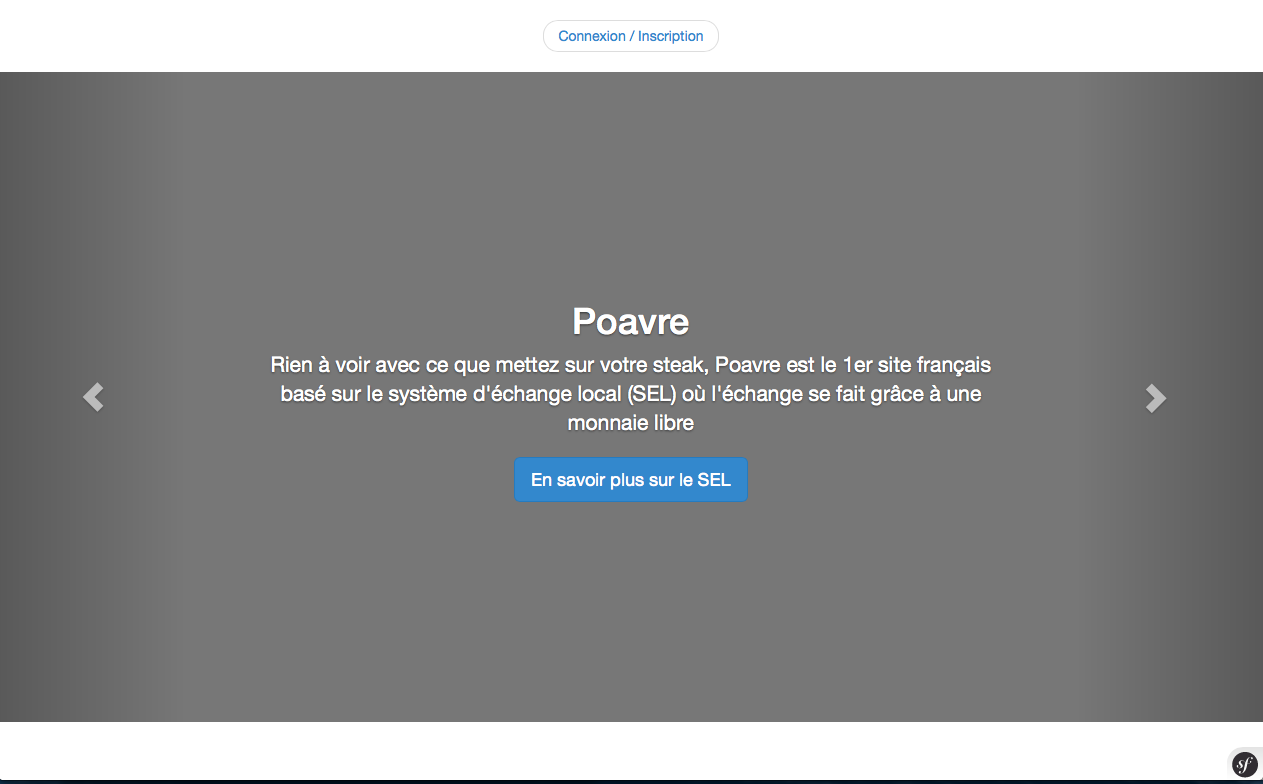
\includegraphics[width=1.0\textwidth]{cap1}
\caption{Page d'accueil du site}
\label{fig:accueil_site}
\end{figure}

%rajouter partie headerbar

\subsection{Choix du langage}
% auteur : Fabien
% relu par : Clément, Florian, Thin

Le choix du langage ou plutôt des langages est apparu naturellement lors de la présentation des différents outils de programmation.

Le PHP est indispensable ainsi que le CSS pour la mise en forme.

Quant au HTML, il sera utilisé au sein des templates Twig ce qui modifie légèrement la syntaxe car Twig ajoute des outils intéressants au niveau des vues.

Du JavaScript et du JQuery semblent utiles pour donner de la vie au site, notamment pour réaliser une page d'accueil dynamique, réactive et attrayante et pour la gestion des droits au sein des groupes ou du site d'une façon plus générale.

Au niveau de la langue, nous avions décidés initialement de réaliser un site cent pour cent anglophone (programmation, commentaires et affichage en anglais), puis finalement, après modification du code réalisé, nous sommes venus à une programmation en anglais, des commentaires en anglais mais un affichage en français car les utilisateurs finaux sont français.

\subsection{Choix du framework}
% auteur : Fabien
% relu par : Clément, Florian, Thin

Tout d'abord, nous avons établis qu'un framework serait plus judicieux pour la réalisation de ce projet c'est pourquoi les CMS présentés n'ont pas été retenus.

Aussi, nous voulions un framework puissant, mettant à notre disposition des fonctions utilisables pour notre projet afin de nous faciliter la programmation. Nous recherchions également un framework que nous pourrions utiliser à court terme, dans notre vie professionnelle.

CakePHP étant peu utilisé dans les entreprises françaises il n'a pas retenu notre attention. Il en va de même pour FuelPHP qui n'est quasiment pas utilisé en France. Finalement et avec enthousiasme Symfony2 a été choisi à l'unanimité pour ses performances, ses tutoriels mis à disposition (voir \cite{tuto_symfony}) et par sa forte utilisation au sein des entreprises françaises.

\subsection{Choix du serveur}
% auteur : Fabien
% relu par : Adrien, Clément, Florian, Thin

Au niveau de l'hébergement du site web il nous fallait un hébergeur acceptant une version récente de PHP, qui intégrait facilement des projets Symfony2 et qui donnait les pleins pouvoirs sur le projet de l'extérieur.

Nous avons tout d'abord pensé que nous pourrions héberger le site sur le serveur possédé par notre tuteur mais ce dernier ne s'est pas révélé compatible avec notre projet. Aussi, l'un des membres du projet ayant réalisé un projet avec Symfony2 antérieurement, nous avons décidé d'héberger notre site sur le même serveur à savoir celui de l'hébergeur Hostinger (voir \cite{hostinger}).

Ainsi, nous disposons d'un accès FTP (File Transfert Protocol) pour le transfert des fichiers vers le serveur, d'un accès à PHPMyAdmin qui stocke la base de données, d'une adresse mail propre au projet associée à l'hébergeur et de divers outils pratiques mais pas toujours utiles.

Ce serveur n'est pas dédié pour des raisons pécuniaires, il est donc partagé, mais les performances sont tout de même très bonnes et le site est accessible en tout temps.

\subsection{Choix du gestionnaire de projet et du gestionnaire 
de versions}
% auteur : Fabien/Adrien
% relu par : Clément, Quentin, Thin

\subsubsection{Le gestionnaire de projet}

Un outil de gestion de projet s'est révélé indispensable pour une réalisation efficace de ce projet. Il semblait important que celui-ci permette de gérer les différentes tâches de façon lisible et ordonnée.

Notre tuteur nous a présenté Producteev (voir figure \ref{fig:ScreenProducteev}), un outil de gestion de tâches en ligne et gratuit nous permettant de créer des tâches en spécifiant les collaborateurs leurs étant assignés ainsi que des «~suiveurs~» , afin que ces derniers soient informés par mail de leur avancée. Une échéance et une priorité peuvent être apposées sur les tâches et des sous-tâches qui peuvent également être commentés.

\begin{figure}[ht]
\centering
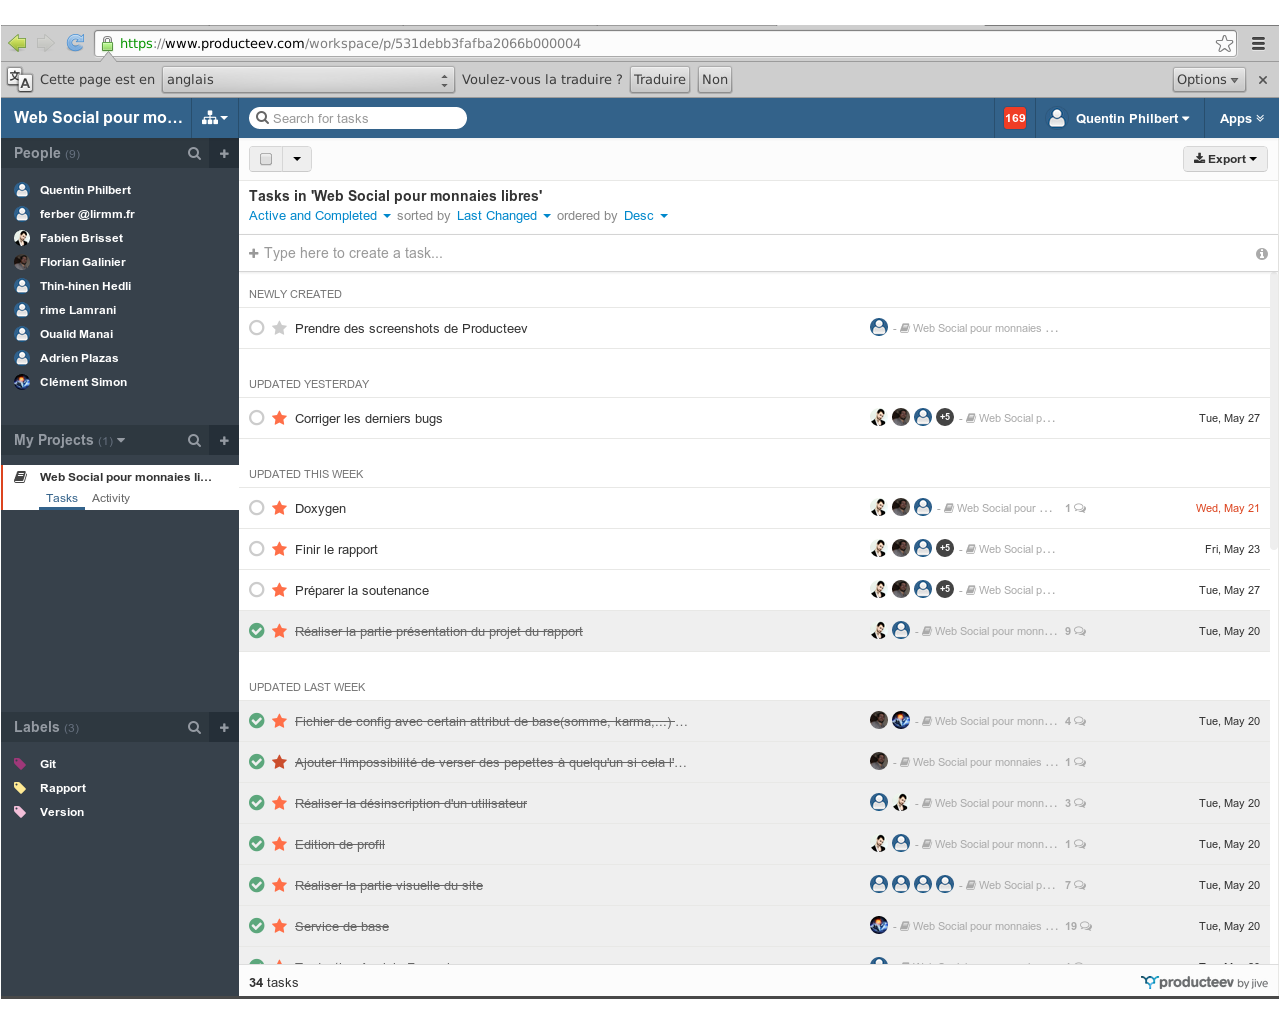
\includegraphics[width=0.9\textwidth]{ScreenProducteev}
\caption{Capture d'écran de Producteev}
\label{fig:ScreenProducteev}
\end{figure}

Le nombre de collaborateurs sur ce gestionnaire de tâche étant illimité, cet outil avec ses fonctionnalités est celui que nous avons choisi pour ce projet. En effet, nous ne nécessitions pas plus de fonctionnalités que celles-ci, nous n'avons donc pas cherchés d'autres outils pour la gestion des tâches du projet.

\subsubsection{Le gestionnaire de versions}

Un gestionnaire de versions semblait nécessaire afin de collaborer efficacement. Le gestionnaire de version distribué Git a rapidement été proposé, en association à Github (voir \cite{github}) pour l'hébergement du code du projet (voir \cite{progit}).
Après analyse des avantages et inconvénients par rapport à un système de gestion de versions centralisé comme SVN, notamment sur l'utilisation des branches, Git et Github ont été retenus.

\begin{figure}[ht]
\centering
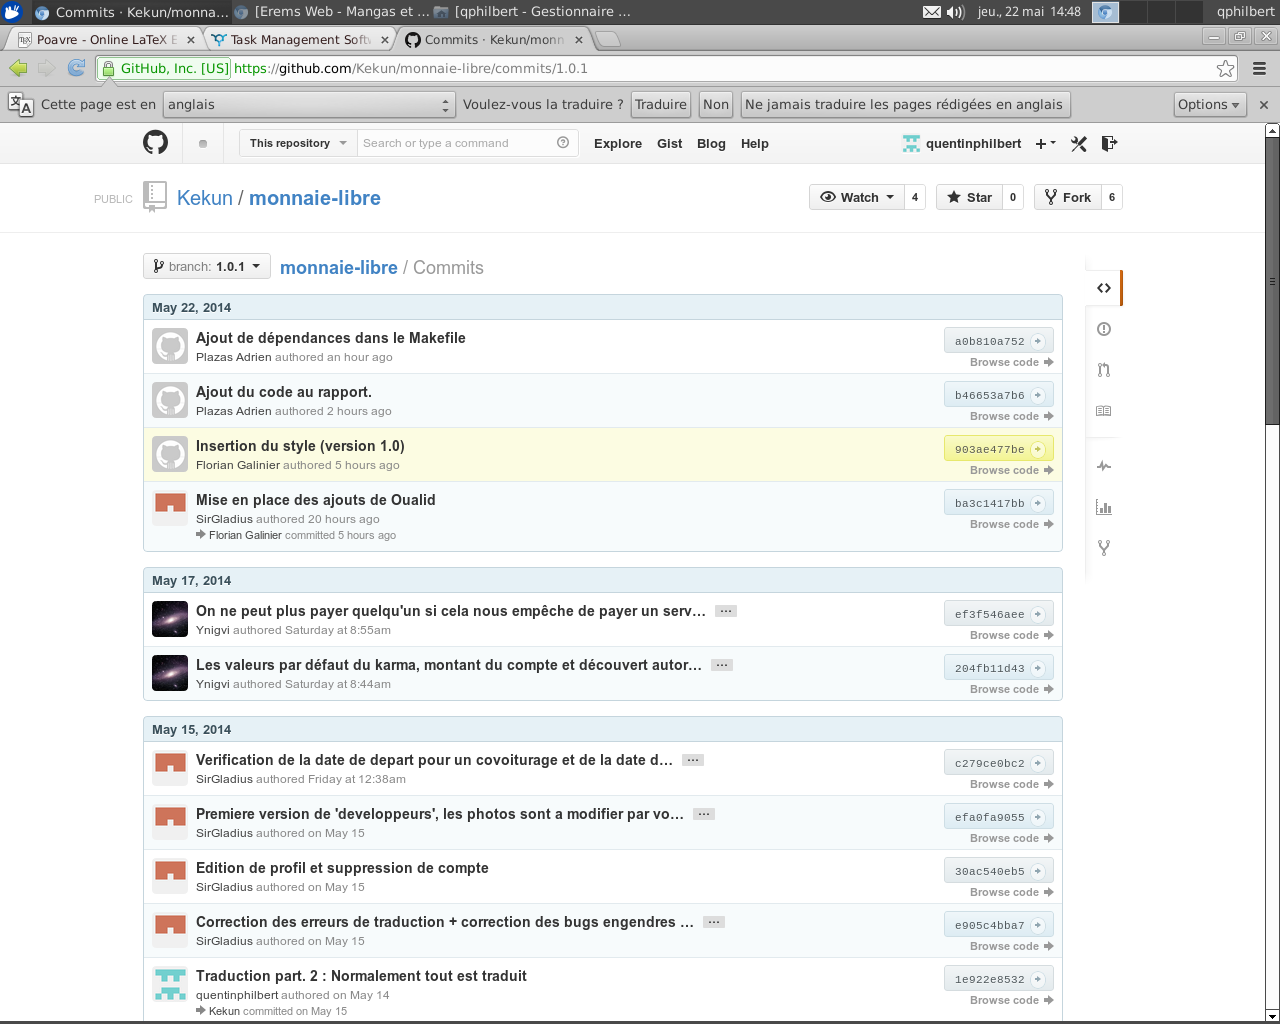
\includegraphics[width=0.9\textwidth]{ScreenshotGITHUB}
\caption{Capture d'écran de GitHub}
\label{fig:ScreenGitHub}
\end{figure}

\paragraph{Avantages}
Git est un gestionnaire de version très utilisé et il est apprécié pour sa robustesse, ses performances, sa praticité et sa capacité de mise à l'échelle (Git gère les versions du noyau Linux, une énorme base de code avec des milliers de collaborateurs).
De plus, cet outil est utilisable en lignes de commande sur de très nombreux systèmes d'exploitation (de Windows à Haiku en passant par Android).

\paragraph{Inconvénients}
Il demande à l'équipe d'apprendre de nombreux nouveaux concepts et son utilisation sur Windows peut être laborieuse, de par son interface en ligne de commande.

\subsection{Choix des outils de documentation}
% auteur : Adrien
% relu par : Fabien, Clément, Thin

Doxygen (voir \cite{doxygen}) est apparu comme un choix évident pour la documentation~:
\begin{itemize}
    \item c'est un logiciel libre, solide et puissant~;
    \item il n'est pas spécifique à un langage et fonctionne bien avec PHP~;
    \item il est assez simple à appréhender~;
    \item sa syntaxe est simple et lisible telle quelle comme documentation dans le code, le rendant assez peu intrusif.
\end{itemize}
Il répond parfaitement à nos besoins de documentation et il n'est pas étonnant qu'il soit devenu un leader dans son domaine.
